\documentclass[11pt]{article}
\usepackage[a4paper,margin=1in]{geometry}
\usepackage{amsmath,amssymb,amsthm,mathtools}
\usepackage{graphicx}
\usepackage{xcolor}
\usepackage{microtype}
\usepackage{enumitem}
\usepackage[colorlinks=true,linkcolor=blue!55!black,citecolor=blue!55!black,urlcolor=blue!55!black]{hyperref}
\setlength{\emergencystretch}{1em}

\newtheorem{theorem}{Theorem}
\newtheorem{proposition}[theorem]{Proposition}
\newtheorem{lemma}[theorem]{Lemma}
\theoremstyle{definition}
\newtheorem{definition}[theorem]{Definition}
\newtheorem{remark}[theorem]{Remark}

\newcommand{\C}{\mathbb C}
\newcommand{\N}{\mathbb N}
\newcommand{\Orb}{\operatorname{Orb}}
\newcommand{\dist}{\operatorname{dist}}

\title{Tail-universal scalar sets for nonunit adjoint eigenvalues}
\author{Candidate partial result for arXiv:1509.04912}
\date{9 August 2026}

\begin{document}
\maketitle

\begin{center}
\fcolorbox{blue!55!black}{blue!4}{\parbox{0.91\linewidth}{
\textbf{Status.} Candidate substantial partial result, likely valid; human
review recommended. The theorem gives a uniform positive answer under an
explicit scalar-set condition in the nonunit-eigenvalue regime. It does not
classify all scalar sets and therefore does not fully solve Question~3.}}
\end{center}

\section{Source problem}

The source is S.~Charpentier, R.~Ernst, and Q.~Menet,
\emph{$\Gamma$-supercyclicity}, arXiv:1509.04912 \cite{CEM}. For a bounded
operator $T$ on a complex Banach space $X$, a vector $x$ is
$\Gamma$-supercyclic when
\[
  \Orb(\Gamma x,T)=\{\gamma T^n x:\gamma\in\Gamma,\ n\geq0\}
\]
is dense in $X$. Question~3 asks which $\Gamma\subset\C$ make
supercyclicity equivalent to $\Gamma$-supercyclicity.

\begin{figure}[ht]
  \centering
  
\includegraphics[width=\linewidth]{figures/open_problem_crop.png}
  \caption{Question~3 on page 3 of the source paper.}
\end{figure}

The source completely treats adjoint eigenvalues of modulus one in
Theorem~C(1), gives a warning example for nonunit eigenvalues in
Theorem~C(2), and then explicitly says that the nonunit and empty-spectrum
cases remain unclear.

To avoid a convention-dependent conjugation, the result below is stated using
an \emph{eigenfunctional multiplier}: $f\circ T=\mu f$. Under the
complex-linear dual convention this is exactly $T^*f=\mu f$; under the
conjugate-dual convention used in the source, the corresponding adjoint
eigenvalue is $\overline\mu$. In either convention the modulus is unchanged.

\begin{figure}[ht]
  \centering
  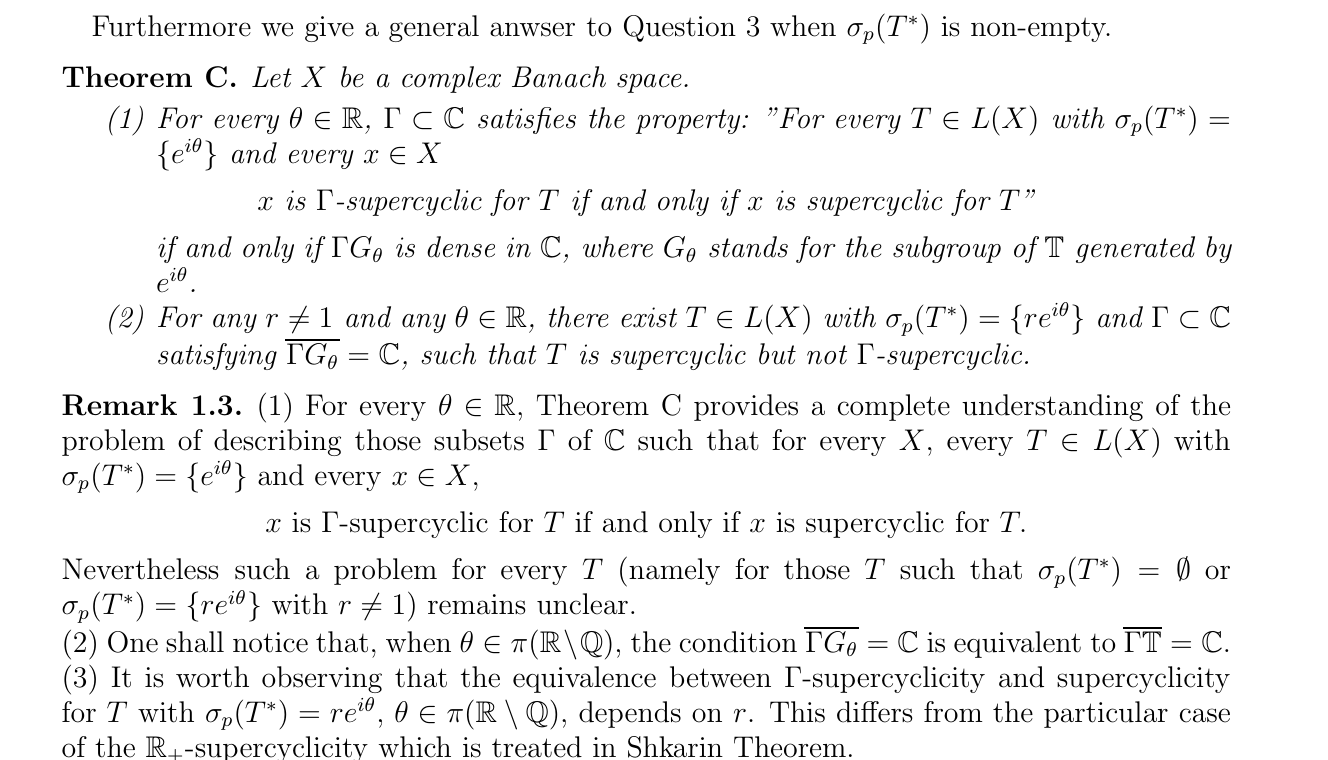
\includegraphics[width=\linewidth]{figures/residual_case_crop.png}
  \caption{Theorem~C and the unresolved nonunit case on page 4 of the source.}
\end{figure}

\clearpage
\section{Proof intuition}

Suppose $f\circ T=\mu f$. A projective approximation
$\alpha_kT^{n_k}x\to y$ is visible through $f$ as
$\alpha_k\mu^{n_k}f(x)\to f(y)$. Thus, for targets outside the
hyperplane $\ker f$, the correct projective coefficient is asymptotically
determined after multiplication by $\mu^{n_k}$. If the rescaled sets
$\mu^n\Gamma$ approach every scalar at every sufficiently late time,
one can replace $\alpha_k$ by coefficients from $\Gamma$ without changing
the vector limit. The source's phase-group condition does not provide this
time synchronization when $|\mu|\ne1$; tail universality does.

The condition is nonvacuous and does not merely say that $\Gamma$ is dense.
Place a finer and larger finite lattice $F_n$ at scale $\mu^{-n}$.
After multiplication by $\mu^n$ the $n$th block becomes $F_n$, while in
the original scale the blocks either collapse to zero or escape to infinity
when $|\mu|\ne1$.

\section{Tail-universal scalar sets}

\begin{definition}
Let $\mu\in\C\setminus\{0\}$. A set $\Gamma\subset\C$ is
\emph{tail-universal for $\mu$} if
\begin{equation}\label{eq:tail}
  \forall c\in\C,\qquad \dist(c,\mu^n\Gamma)\longrightarrow0
  \quad(n\to\infty).
\end{equation}
\end{definition}

\begin{lemma}[Projective tails]\label{lem:tails}
If $x$ is a supercyclic vector for $T$, then for every $N\geq0$,
\[
 \bigcup_{n\geq N}\C T^n x
\]
is dense in $X$.
\end{lemma}

\begin{proof}
The one-dimensional case is immediate. Assume $\dim X>1$. If some
nonempty open set $U$ missed the displayed tail, then density of the full
projective orbit would imply that every nonempty open subset of $U$ meets
the finite union $\bigcup_{n<N}\C T^n x$. Hence this finite union of closed
one-dimensional subspaces would be dense in $U$, and therefore would contain
$U$. A finite union of proper linear subspaces has empty interior, a
contradiction.
\end{proof}

\begin{theorem}[Uniform spectral transfer]\label{thm:transfer}
Let $X$ be a complex Banach space, $T\in\mathcal L(X)$, and suppose that
$f\circ T=\mu f$ for some $f\in X^*\setminus\{0\}$ and
$\mu\ne0$. If $\Gamma$ is tail-universal for $\mu$, then, for
every $x\in X$,
\[
 x\text{ is supercyclic for }T
 \quad\Longleftrightarrow\quad
 x\text{ is $\Gamma$-supercyclic for }T.
\]
\end{theorem}

\begin{proof}
The reverse implication is immediate because $\Gamma\subset\C$. Suppose
that $x$ is supercyclic. Then $f(x)\ne0$, since otherwise
$f(T^n x)=\mu^n f(x)=0$ for every $n$ and the projective orbit would lie
in the proper closed hyperplane $\ker f$.

Fix $y\in X$ with $f(y)\ne0$. By Lemma~\ref{lem:tails}, there are integers
$n_k\geq k$ and scalars $\alpha_k$ such that
\[
  \alpha_kT^{n_k}x\longrightarrow y.
\]
Applying $f$ and dividing by $f(x)$ gives
\[
  \alpha_k\mu^{n_k}\longrightarrow
  c:=\frac{f(y)}{f(x)}\ne0.
\]
By \eqref{eq:tail}, choose $\gamma_k\in\Gamma$ with
$\gamma_k\mu^{n_k}\to c$. Since both scaled coefficient sequences
converge to the same nonzero number,
\[
 \frac{\gamma_k}{\alpha_k}
 =\frac{\gamma_k\mu^{n_k}}{\alpha_k\mu^{n_k}}
 \longrightarrow1.
\]
Consequently $\gamma_kT^{n_k}x\to y$. Thus the closure of
$\Orb(\Gamma x,T)$ contains $X\setminus\ker f$, which is dense in $X$.
\end{proof}

\section{Countable non-dense examples}

\begin{proposition}\label{prop:lattice}
For every $\mu\in\C\setminus\{0\}$ with $|\mu|\ne1$, there is
a countable non-dense set $\Gamma_\mu\subset\C$ that is
tail-universal for $\mu$. One explicit choice is
\[
 F_n=\left\{\frac{j+ik}{n}:j,k\in\mathbb Z,\ j^2+k^2\leq n^4\right\},
 \qquad
 \Gamma_\mu=\bigcup_{n\geq1}\mu^{-n}F_n.
\]
\end{proposition}

\begin{proof}
Fix $c\in\C$. Round $n\Re c$ and $n\Im c$ to nearest integers $j_n$ and
$k_n$. For all sufficiently large $n$,
$j_n^2+k_n^2\leq n^4$, so
$q_n=(j_n+ik_n)/n$ belongs to $F_n$, and
\[
 |q_n-c|\leq\frac{\sqrt2}{2n}.
\]
Because $F_n\subset\mu^n\Gamma_\mu$, condition
\eqref{eq:tail} follows.

It remains to prove non-density. Write $r=|\mu|$. If $r>1$, the
$n$th block $\mu^{-n}F_n$ is contained in the disk of radius
$nr^{-n}$, which tends to zero. Apart from the common point zero, only
finitely many blocks can meet any fixed annulus bounded away from zero, so
the union is not dense. If $0<r<1$, every nonzero point of the $n$th block
has modulus at least $r^{-n}/n$, which tends to infinity. Hence every
bounded disk contains nonzero points from only finitely many finite blocks,
and again the union is not dense. Countability is immediate.
\end{proof}

\begin{remark}
Combining Theorem~\ref{thm:transfer} and Proposition~\ref{prop:lattice}
gives, for each nonunit $\mu$, a single countable non-dense scalar set
that works simultaneously for every supercyclic operator possessing the
adjoint spectral multiplier $\mu$ and for every one of its supercyclic vectors.
This is stronger than constructing a set for one selected operator.
\end{remark}

\section{Verification, novelty, and limitations}

The proof is analytic. The accompanying checker verifies finite lattice
rounding errors and the two block-scale asymptotics for representative
eigenvalues on either side of the unit circle. These computations are
sanity checks only.

A bounded search on 9 August 2026 covered:
\begin{itemize}[nosep,leftmargin=1.4em]
\item the run indexes and the source paper;
\item arXiv:1711.10932, arXiv:2005.11230, and arXiv:2411.03179;
\item exact or close searches for \emph{$\Gamma$-supercyclicity},
  \emph{nonunit adjoint eigenvalue}, \emph{$\mu^n\Gamma$}, and
  \emph{scaled scalar sets}.
\end{itemize}
No explicit version of Theorem~\ref{thm:transfer} or
Proposition~\ref{prop:lattice} was found. Novelty confidence is moderate.

The result is partial: condition \eqref{eq:tail} is sufficient, but no
necessity theorem is claimed; the source's empty adjoint point-spectrum case
also remains open. Human review should focus on Lemma~\ref{lem:tails}, the
coefficient-ratio step in Theorem~\ref{thm:transfer}, the non-density proof,
and the bounded novelty assessment.

\begin{thebibliography}{9}
\bibitem{CEM}
S.~Charpentier, R.~Ernst, and Q.~Menet,
\emph{$\Gamma$-supercyclicity}, Integral Equations Operator Theory
85 (2016), 71--92; arXiv:1509.04912.
\end{thebibliography}

\end{document}
